\documentclass{standalone}
\usepackage{tikz}
\usepackage{pgfplots}
\usepackage{amsmath}
\pgfplotsset{compat=1.18}

\begin{document}
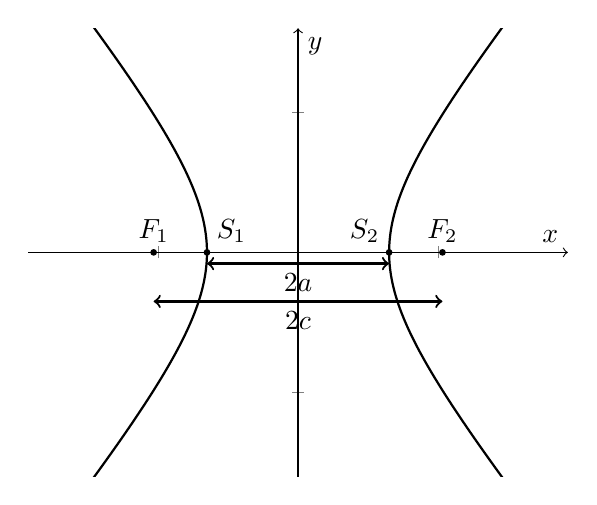
\begin{tikzpicture}[scale=1]
\begin{axis}[
    xmin=-17, xmax=17,
    ymin=-16, ymax=16,
    axis lines=middle,
    axis line style={->},
    ticklabel style={font=\tiny},
    axis equal,
    xticklabels=\empty,
    yticklabels=\empty,
    xlabel={$x$},
    ylabel={$y$},
]

% Parameters
\def\a{6.5}
\def\b{8}
\pgfmathsetmacro{\c}{sqrt(\a*\a+\b*\b)}

% Right branch of hyperbola
\addplot [domain=0:1.8, samples=100, thick] 
    ({\a*cosh(x)}, {\b*sinh(x)});
% Left branch of hyperbola
\addplot [domain=0:1.8, samples=100, thick] 
    ({-\a*cosh(x)}, {\b*sinh(x)});
    % Right branch of hyperbola
\addplot [domain=0:1.8, samples=100, thick] 
    ({\a*cosh(x)}, {-\b*sinh(x)});
% Left branch of hyperbola
\addplot [domain=0:1.8, samples=100, thick] 
    ({-\a*cosh(x)}, {-\b*sinh(x)});

% Foci
\filldraw (axis cs:\c,0) circle (1pt) node[above] {$F_2$};
\filldraw (axis cs:-\c,0) circle (1pt) node[above] {$F_1$};

% Vertices
\filldraw (axis cs:\a,0) circle (1pt) node[above left] {$S_2$};
\filldraw (axis cs:-\a,0) circle (1pt) node[above right] {$S_1$};



% Double-headed arrows
\draw[<->, thick] (axis cs:-\a,-0.8) -- (axis cs:\a,-0.8) node[midway, below] {$2a$};
%\draw[<->, thick] (axis cs:0,-\b-0.3) -- (axis cs:0,\b+0.3) node[midway, left] {$2b$};
\draw[<->, thick] (axis cs:-\c,-3.5) -- (axis cs:\c,-3.5) node[midway, below] {$2c$};

\end{axis}
\end{tikzpicture}
\end{document}